% This is the root file of your thesis: thesis.tex
% A line starting with % is a comment. In some cases, I have included a command preceded by a %. You may activate the command by removing the %.

%%===================================  packages
\documentclass[12pt]{report}
\usepackage{ramsstyle}
\usepackage[table]{xcolor}
\usepackage{caption}
\usepackage{listings}
\usepackage{graphicx}
\usepackage[normalem]{ulem}
\usepackage[section]{placeins}
\usepackage{mathtools}
\usepackage[T1]{fontenc}
\usepackage[parfill]{parskip}%Begin paragraphs with an empty line rather than an indent

\usepackage{float}
\restylefloat{table}

\usepackage[nottoc,numbib]{tocbibind}%Dispalay refrences in the table of contents

%\renewcommand{\familydefault}{sans}


%%===================================
%Write the various parts of your thesis as separate files and include them into the main file by the command \include{name of included file}. When you compile the LaTeX file, you may choose which subfiles to include by the command

%\includeonly{chapter01,chapter02}

%%===================================
\begin{document}
%%===================================
%This is the Titlepage
%%=========================================
\thispagestyle{empty}
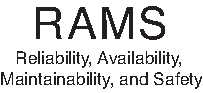
\includegraphics[scale=1.1]{fig/rams}
\mbox{}\\[6pc]
\begin{center}
\Huge{This is the Title of my Thesis}\\[2pc]

\Large{Your Name}\\[1pc]
\large{December 2012}\\[2pc]

PROJECT THESIS\\
Department of Production and Quality Engineering\\
Norwegian University of Science and Technology
\end{center}
\vfill

\noindent Supervisor 1: Professor Ask Burlefot

\noindent Supervisor 2: Professor Fingal Olsson

 % This is the titlepage
\setcounter{page}{0}
\pagenumbering{roman}
%%This is the Preface
%%=========================================
\addcontentsline{toc}{section}{Preface}
\section*{Preface}
Here, you give a brief introduction to your work. What it is (e.g., a Master's thesis in RAMS at NTNU as part of the study program xxx and\ldots), when it was carried out (e.g., during the autumn semester of 2021). If the project has been carried out for a company, you should mention this and also describe the cooperation with the company. You may also describe how the idea to the project was brought up.\\[2cm]

\begin{center}
Trondheim, 2012-12-16\\[1pc]
(Your signature)\\[1pc]
Ola Nordmann
\end{center}
%%This is the Acknowledgment
%%=========================================
\addcontentsline{toc}{section}{Acknowledgment}
\section*{Acknowledgment}
I would like to thank the following persons for their great help during \ldots

If the project has been carried out in cooperation with an external partner (e.g., a company), you should acknowledge the contribution and give thanks to the involved persons.

You should also acknowledge the contributions made by your supervisor(s).

\begin{flushright}
O.N.\\[1pc]
(Your initials)
\end{flushright}
%%This is the Summary
%%=========================================
\addcontentsline{toc}{section}{Summary and Conclusions}
\section*{Summary and Conclusions}
Here you give a summary of your your work and your results. This is like a management summary and should be written in a clear and easy language, without many difficult terms and without abbreviations. Everything you present here must be treated in more detail in the main report. You should not give any references to the report in the summary -- just explain what you have done and what you have found out. The Summary and Conclusions should be no more than two pages.
\tableofcontents
\setcounter{page}{0}
\pagenumbering{arabic}
%This is chapter 1
%%=========================================
\chapter{Introduction}
File recovery from digital data storage devices has been a hot topic among
the Digital Forensics field. Traditional data storage devices make use of a
file system, in order to manage contained data, their available space and to
maintain location of files. When the storage device and their file system are
intact, it is quite simple to recover data from them. This is mainly because
file systems make use of meta-data in order to track information for their
files. Meta-data can contain information such as creation date, data struc-
ture (e.g directory or regular file), file type, file owner, size, last modified
date etc. In a real life forensic case it is highly unlikely that file meta-data will be
present, or they might be corrupted or deleted. It became clear for the digi-
tal forensic community that an alternative, more realistic approach must be
used.

%%=========================================
\section{Background}
File carving is a forensics technique that recovers files based on their content,
without relying on their meta-data. File carving process involves two steps.
File validation and file reconstruction.[1]. During the recovery procedure,
we must first validate the type of the file and then apply the appropriate
reconstruction technique. In this thesis, only the validation techniques are
of our interest.
By examining the content (the actual byte-code) and/or the structure of
a file [22], file validation techniques are used to classify its type. Several file
types contain common structures like headers, footers (named Magic Number
Matching) [7][3], fields that specify file attributes like color or size etc.(Data
Dependency Resolving [3]), that can be used to identify the type of the file.
Additionally, another approach is to apply statistical analysis techniques and
algorithms, which use the complete byte code of a file, creating a fileprint for
every file type. Some examples are the n-Gram Analysis [9], the Byte fre-
quency analysis (BFA) algorithm and the Byte frequency cross-correlation
(BFC)[4].
The aforementioned techniques have some profound weaknesses. The Magic
Number Matching and the Data Dependency Resolving approaches make
general type classification infeasible. This is due to the fact that not every
2file type contains such structures. Furthermore, n-Gram Analysis and both
BFA and BFC were designed to be applied in a complete file or a pre-defined
part of it, which retains all of its content. Hence, they depend on files inter-
nal structure and characteristics.
%%=========================================
\subsection*{Problem Formulation}
So why this is a problem? The answer lies in file systems behaviour and
file fragmentation. When we delete a file from a media storage, the data are
not actually removed. The clusters in which the file was stored still contain
the same data, although the file system mark them as unallocated [2]. Which
means that the next time a new file is created, the file system is free to use
these clusters, which are marked as unallocated, to store the new file. But
if the new file is bigger than the old one, and the file system tries to store it
starting from the same cluster entry as the deleted one, it wont have enough
space to store it. So the file system will allocate all the clusters of the previ-
ous deleted file, while the remaining data which do not fit, will be stored to
other unallocated clusters. This results to file fragmentation. In a forensic
file recovery case, it is more probable that the files that must be recovered are
fragmented. Validation techniques which use the complete file content
are high unlikely to provide aid to forensic examiners. Hence, an alternative
approach to file type validation must be taken.
File fragment classification is a technique that uses only a small fragment
of a file, in order to determine its type. Ergo, file fragmentation is not a
problem any more as this approach is independent from files overall struc-
ture. Although in theory file fragment classification looks like an ideal so-
lution, in practice current solutions that use this approach could not yield
good results[6][22]. One reason that file fragment classification is difficult, is
due to the complex container files. Complex container files like TAR, ZIP,
RAR, PDF etc. contain other primitive file types, making general fragment
classification difficult. Moreover, a fragment might contain more data which
are strongly related to the files content than the files structure
%%=========================================

%%=========================================
\section{Objectives}
Although general fragment classification is difficult (due to lots of file formats containing large blocks of highly compressed data that look similar to a classifier), a large amount of file types consist of or at least contain, (plain) text data. In this project our main objectives are
\begin{enumerate}
\item This is the first objective
\item This is the second objective
\item This is the third objective
\item More objectives
\end{enumerate}




%%=========================================
\section{Approach}
 It has been observed that BFA, although extremely inaccurate, classifies a big amount of fragments that belong to a document file as text. We will make use of the classic BFA among with some variations of it and try to enhance its accuracy on classifying document-file fragments as text. Then we will isolate all the fragments classified as text and analyse them in order to find patterns which will help us to design our algorithm. The BFA that we are going to use is the same as [McDaniled] with the only difference that we wont train our fingerprints with the complete byte set of the fragments. Due to the fact that many file types contain partially plain text, in this
project we will analyse the byte set that corresponds to printable ASCII
characters ( 32  b  126 ) of every fragment. Additionally, some more bytes
that could reveal a documents nature as the newline (10), tab (9), carriage re-
turn (13) characters are being used. Until now, almost
every approach, for both file and fragment classification, analyses the complete ASCII byte set (0..255). We will try to discover if by ignoring
almost half of the ASCII byte set, we can acquire more reliable results and create an algorithm which will be able to classify document-type file fragments with better accuracy. Moreover, after the design and implementation of our algorithm, we are going to use
the same corpus as Shahi did in [XX] in order to test effectively the accuracy of our algorithm. 



%%=========================================
\section{Structure of the Report}
The rest of the report is structured as follows. Chapter 2 gives an introduction to \ldots

\begin{remark}
Notice that chapter and section headings shall be written in lowercase, but that all main words should start with a capital letter.
\end{remark}


The report should be no longer than \underline{60 pages} in this format (+ the CV).
\chapter{Related Work}

\section{Related Work}
Karresand and Shahmehri~\cite{roc} introduced a new algorithm that uses a metric called Rate-of-Change (ROC). They define the rate of change of a byte content as the difference of the ASCII values of consecutive bytes. Although this technique yields good classification rates for jpeg files (99\% true positives), mainly because of their 0xFF00 metadata tags, for other files types the false positive rates are extremely high ( e.g for zip and portable executable(PE) files near 70\% false positives rates).

Veenman\cite{Veenman} used a combination of the BFA\cite{MacDaniel} with Shannon entropy and Kolmogorov complexity measures to classify fragments that were 4096 bytes in size. He used a corpus of 450mb comprised of 11 different file types. He managed to achieve high detection rates(99\%) for jpeg and html files. However, results for the other file types weren't so good, achieving an overall acurracy of 45\%. Additionally, the corpus that he used is not big enough to produce statistically significant results. Moreover, the big size of the fragments that Veenman used is not convenient enough for a real forensic case.

Calhoun  and Coles~\cite{Calhoun} used a set of techniques like byte frequency of ASCII codes and Shannon entropy, linear discriminant analysis and prediction with longest common substrings and subsequences along with many other common statistical metrics. Their corpus was comprised of gif, pdf, jpeg and bmp files.
Although they achieved a high average rate of correct prediction of 88.3\%, their testing set was comprised only of 50 fragments per file type. The fragments size that were used in their experiment was of 512 and 896 bytes. Moreover, since they don't give information about the lengths of the file type representative strings  that were used, we don't know how expensive longest common subsequence technique can be. 

Axelsson\cite{Axelsson} used a corpus of 28 different file types and applied the k-nearest-neighbour classification technique with Nearest Compression Distance(NCD) as the distance metric between file fragments. The results are unremarkable, achieving an average accuracy of around 34\%. It was observed that this approach achieved higher accuracy for fragments with high entropy.

%Gopal, Yang, Salomatin and Carbonell\cite{Gopal} used several statistical classification methods, such as support vector machines with n-gram feature vectors, and k-nearest-neighbours with cosine similarity as the distance metric. They combined these techniques with several commercial off-the-shelf solutions (e.g Outside- In, Libmagic, DROID and TrID) in classifying files under various scenarios. Many important information are not reported for this research such as the classifiers performance for each file type. It is known that they achieved an accuracy of 33\% using the macro-averaged F1 measure [25].

Fitzgerald, Mathews, Morris and Zhulyn\cite{Fitz} investigated whether techniques from natural language processing could be applied successfully to file fragment classification. They used the macro-averaged F1 metric in a set of 24 file types. They managed to achieve an average prediction accuracy of 49.1\% on 24 file types out performing Axelssons (34\% for 28 file types) and Veenmans (45\% for 11 file types) results.

Lastly, Shahi\cite{Ashim} tested 4 different classification algorithms in the same corpus, in order to compare their performance. His corpus was comprised of 10 different file types. The algorithms used were the BFA\cite{MacDaniel}, the N-Gram Analysis\cite{ngram}, the Rate of Change\cite{roc} and the algorithm of Conti et al.~\cite{Conti}. The results show that the average overall accuracy of the aforementioned techniques is around 30\%. Moreover he benchmarked their performance in terms of execution time and found out that the N-Gram Analysis is the fastest among them, with BFA coming second, third the Rate of Change and fourth the algorithm of Conti et al.





\chapter{Experimental Setup}


\section{Data Set}
The data set we used for both our training and testing procedures is derived from  Garfinkels[] coprus, Wikipedia and Academic Earth[] and is the exact same coprus that Shahi[] used for his testing set.The set is comprised of 10 different file types with a size of about 1GB each. We split this corpus in a 9-1 ratio for the training and testing set respectively. 
Furthermore, we divided both the testing and training set files in 512-byte blocks, which we refer to them as fragments. We used the training set to train our fingerprints and apply statistical analysis in order to discover useful patterns and the testing set to test all variations of our BFA algorithm. More detailed information about our data set can be found in Table ~\ref{table:data set}.
%%------------------------------------------------------------------------------------------------------------------------------
\begin{table}
\centering
\caption{Experimental Data Set\label{table:data set}}
\colorbox{blue!30}{
\scalebox{0.62}{

\begin{tabular}{ l r r r r r r r r r r }
\hline
\hline
 & pdf  &  zip  &  text  &  doc  &  mp4  &  xls  &  ppt  &  jpg  &  ogg  &  png \\ [0.6ex]
\hline\\
\uline{Training Set} \\[0.6ex]
num.of files                               & 1,642    & 1        & 954      & 1,697    & 1        & 373      & 193      & 1,781    &464   & 4,395    \\[0.6ex]
size in megabytes                          & 869.3	 & 860.6    & 831.2    & 867.6    & 813.6    & 869.5    & 866.9    & 870.5    &863.4 & 868.9 \\[0.6ex]
expected num. of fragments                 & 1,780,326& 1,762,508& 1,702,297& 1,776,844& 1,666,252& 1,780,736& 1,775,411& 1,782,784&1,768,243 &1,779,507    \\[0.6ex]
output num.of fragments                    & 1,694,034& 1,680,771& 1,622,534& 1,467,314& 1,588,908& 1,684,374& 1,683,444& 1,698,877&1,685,954 &1,692,813    \\[0.6ex]  
percentage of fragments with no plain text & 4.8	     & 4.6      & 4.7      & 17.4     & 4.6      & 5.4      & 5.2      & 4.7      &4.7   &4.9  \\\\\\

\uline{Testing Set} \\[0.6ex]
num.of files                               & 217	   & 1      & 367    & 257    & 1      & 81     & 35     & 214    & 101    & 555    \\[0.6ex]
size in megabytes                          & 100	   & 104.9  & 97.4   & 100.2  & 104.9  & 100.2  & 100.6  & 100.2  & 100.2  & 101.5    \\[0.6ex]
expected num. of fragments                 & 204,800& 214,835& 199,475& 205,209& 214,835& 205,209& 206,028& 205,209& 205,209& 207,872    \\[0.6ex]
output num.of fragments                    & 189,732& 204,795& 190,055& 177,887& 204,728& 193,352& 195,289& 195,608& 195,656& 195,653   \\[0.6ex]
percentage of fragments with no plain text & 7.4    & 4.7    & 4.7    & 13.3   & 4.7    & 5.8    & 5.2    & 4.7    & 4.7    & 5.9 \\

\end{tabular}}}
\end{table}



\section{Byte Frequency Analysis(BFA) Algorithm}
BFA [McDaniels] is a statistical learning algorithm that was initially developed to analyse and classify whole files. It was not meant to be used in file fragments. By counting the number of instances of each byte in a file of a certain type, BFA uses this frequencies to create a representative average value for each byte instance, among with their respective correlation strength. This results in a fingerprint for this particular file-type. Then during the classification procedure, the input file is compared with every fingerprint and an accuracy level is created for each file type. BFA classifies the file to the file type that corresponds to the highest accuracy level.
 Shahi trained and tested BFA with file fragments of 512-byte size and his results show that although the algorithm is pretty bad for broad fragment classification, it is quite good in identifying fragments that belong to document-type files as text. We use a BFA which will train our fingerprints with the bytes that corresponds to the printable ASCII characters plus the tab, line break and carriage return instead of the complete byte-set of the fragments. This BFA will be only the first step of our algorithm and we intend to use additional metrics after this point. Taking under account the speed requirements, BFA seems as a very good candidate since it is quite a lightweight technique compared to heavier machine learning algorithms. Moreover, as we already stated, BFA seems to classify a big ammount of document-type fragments as text. Shahi tested several classification algorithms in the same corpus. BFA was also tested among with Byte Frequency Correlation algorithm, n-Gram Analysis and Conti et al. algorithm. The results show that BFA has the highest precision in classifying document-type fragments as text.




\chapter{BFA Variations}

\section{Variation 1 - Special ASCII subset fingerprint training}

In this variation we created 10 fingerprints which were trained with fragments from the training set, one for each file type. We used only the printable ASCII characters (32 $\geq$  b $\leq$ 126) among with the tab(9), new line (10) and the carriage return(13) characters. The results can be found in Table \ref{table:table 4.1}.\\\\
 This variation of BFA classifies 589,758 fragments as text which corresponds to the 30.4\% of the initial corpus. 501,012 of them are fragments that come from pdf, xls, doc and text files and 88,746 fragments originate from the other 6 file types. This means that in the set that is classified as text we have an 85\% of true positives in identifying document-type fragments as text with 15\% false positives. This 85\% of true positives corresponds to the 66.7\% of the total pdf, xls, doc and text files of our corpus.

%%------------------------------------------------------------------------------------------------------------------------------

\begin{table}
\centering
\caption{BFA Results - Fingerprints with printable ASCII characters\label{table:table 4.1} }

\colorbox{blue!30}{
\scalebox{0.65}{

\begin{tabular}{ l c c c c c c c c c c }
\hline
\hline
 & pdf  &  zip  &  text  &  doc  &  mp4  &  xls  &  ppt  &  jpg  &  ogg  &  png \\ 
\hline
num.of fragments  & 189,732	 &  204,795  & 190,055  & 177,887  & 204,728  & 193,352  & 195,608  & 195,608  & 195,656  & 195,653   \\[0.6ex]
\hline
\\[0.2ex]
pdf 		 & \cellcolor{blue!15}27.9  & 52.3  & 0.0 & 20.3  & 48.1 & 0.2 & 35.3 & 40.7  & 46.5  & 44.1   \\[0.6ex]
zip 		 & 20.2 & \cellcolor{blue!15}26.6  & 0.0  & 13.3  & 28.0 & 0.1 & 24.9 & 29.2  & 24.7  & 28.2   \\[0.6ex]
\rowcolor{blue!50}
\cellcolor{blue!30}text		 & 21.3 & 4.9  & \cellcolor{blue!15}98.0 & 50.4  & 4.4   & 95.5  & 14.1 & 6.0 & 7.1   & 7.2   \\[0.6ex]
doc 		 & 14.4 & 4.2  & 0.5  & \cellcolor{blue!15}7.1  & 5.2 & 0.2  & 9.7  & 7.9  & 8.7  & 5.8   \\[0.6ex]
mp4 		 & 1.7 & 0.6  & 0.0  & 0.2  & \cellcolor{blue!15}0.8  & 0.0  & 0.4  & 0.5  & 0.4  & 0.5   \\[0.6ex]
xls 		 & 1.2 & 0.0  & 1.4  & 0.8  & 0.1  & \cellcolor{blue!15}3.9  & 1.0  & 0.2  & 0.0  & 0.1   \\[0.6ex]
ppt 		 & 3.2 & 2.2  & 0.0  & 1.8  & 2.7  & 0.0  &  \cellcolor{blue!15}3.3  & 3.3 & 2.7  & 2.9   \\[0.6ex]
jpg 		 & 0.5 & 0.1  & 0.0  & 0.1  & 0.0 & 0.0  & 0.1  & \cellcolor{blue!15}0.1  & 0.0  & 0.1   \\[0.6ex]
ogg 		 & 2.8 & 2.2  & 0.0  & 1.4  & 3.0 & 0.0  & 2.8  & 3.0  & \cellcolor{blue!15}2.7  & 2.7   \\[0.6ex]
png 		 & 6.8 & 6.9  & 0.0  & 4.6  & 7.7 & 0.0  & 8.3  & 9.1  & 7.2  & \cellcolor{blue!15}8.5   \\[0.6ex]
Unclassified  &  0.0  & 0.0  & 0.0  & 0.0  & 0.0  & 0.0  & 0.0  & 0.0  & 0.0  & 0.0   \\[0.6ex]

\end{tabular}}}
\end{table}

%End table -BFA FULL Fingerprints


\section{Variation 2 - 4-Ratio categories of our special ASCII subset}
During our research we thought that it would be interesting to analyse the distribution of bytes that belong to our special ASCII subset of the training set fragments. Depending on the percentage of our special ASCII subset in a fragment, the fragment was assigned to one of 4 ratio categories. 0-25\%, 25-50\%, 50-75\% and 75-100\%. The results of this analysis can be found in Table ~\ref{table:table 4.2}. As it seems fragments from certain file types are more likely to belong to certain ratio categories. For example almost all text fragments(99.95\%) contain more than 75\% of our special ASCII subset and almost all xls fragments less than 50\%. Undoubtedly this is completely reasonable. Text files are mostly comprised of plain text and Excel sheets, with their cell-like structure, contain less printable characters. And this analogy is more obvious in a 512-byte fragment. That finding can be used as a metric to improve current classification techniques and we are going to elaborate more on this later in this document.\\
\begin{table}[!b]
\centering
\caption{Training Set Ratio of special ASCII subset Analysis\label{table:table 4.2} }
\colorbox{blue!25}{
\scalebox{0.75}{
\begin{tabular}{ l c c c c c c c c c c }
\hline
\hline
ratio & pdf  &  zip  &  text  &  doc  &  mp4  &  xls  &  ppt  &  jpg  &  ogg  &  png \\ 
\hline

\\[0.2ex]
0 - 25\% 		 & 9,327      & 347        & 235        & 528,661    & 3,130      & 1,054,503  & 114,968    & 7,842      &785    & 11,875    \\[0.6ex]
25 - 50\% 		 & 1,332,849  & 1,680,052  & 436        & 768,686    & 1,585,760  & 576,755    & 1,547,585  & 1,685,320  & 1,684,877  & 1,674,301    \\[0.6ex]
50 - 75\%		 & 86,583     & 370        & 181        & 8,834      & 18         & 31,595     & 10,106     & 1,305      & 287  & 1,787  \\[0.6ex]
75 - 100\%		 & 265,275    & 2          & 1,621,682  & 161,133    & 0          & 21,521     & 10,785     & 4,410      & 5    & 4,850 \\[0.8ex]
Total:	         & 1,694,034  & 1,680,771  & 1,622,534  & 1,467,314   & 1,588,908  & 1,684,374  & 1,683,444  & 1,698,877  & 1,685,954   & 1,692,813 \\[0.6ex]\\


0 - 25\% 		 & 0.55  & 0.02  & 0.01  & 36.03   & 0.20  & 62.61  & 6.83   & 0.46  & 0.05   & 0.70    \\[0.6ex]
25 - 50\% 		 & 78.68 & 99.96 & 0.03  & 52.39   & 99.80 & 34.24  & 91.93  & 99.20 & 99.94  & 98.91   \\[0.6ex]
50 - 75\%		 & 5.11  & 0.02  & 0.01  & 0.60    & 0     & 1.88   & 0.60   & 0.08  & 0.02   & 0.11  \\[0.6ex]
75 - 100\%		 & 15.66 & 0     & 99.95 & 10.98   & 0     & 1.28   & 0.64   & 0.26  & 0      & 0.29   \\[0.6ex]

\end{tabular}}}
\end{table}

Based on the analysis results  we thought that would be interesting to divide the fragments of our training set in 4 such categories. Then for each category and for each file type we created their respective fingerprints. So we ended up with 40 fingerprints, 4 for every file type. The algorithm checks first the ratio of our special ASCII subset of the input fragment and according to its value it compares the fragment with the fingerprints of the respective category. The results of this BFA variation can be found in Tables ~\ref{table:table 4.3}, \ref{table:table 4.4}, \ref{table:table 4.5} and \ref{table:table 4.6}.\\ The accuracy for both the actual classification and the text classification are really bad. This variation classified 366,969 fragments as text which corresponds to the 18.9\% of the initial corpus. 87,837 of them are fragments that come from pdf, xls, doc and text files and 279,132 fragments originate from the other 6 file types. This means that in the set that is classified as text we have an 31.5\% of true positives in identifying document-type fragments as text with 68.5\% false positives. This percentage of true positives corresponds to the 11.7\% of the total pdf, xls, doc and text files of our corpus.\\
\begin{table}[t]
\centering
\caption{BFA - Fingerprints Trained in 0-25\% and tested in 0-25\%\label{table:table 4.3}}
\colorbox{blue!30}{
\scalebox{0.75}{

\begin{tabular}{ l c c c c c c c c c c }
\hline
\hline
 & pdf  &  zip  &  text  &  doc  &  mp4  &  xls  &  ppt  &  jpg  &  ogg  &  png \\ 
\hline
num.of fragments  & \ 5,714 \  &\ \ \ 90 \ \  & \ \ \ \ \ 3 \ \ \  & \ 52,264   &\ 2,854 \  & 147,873   & \ 11,027   & \ 1,332 \   &\ \  222 \ \  & \ 7,874 \   \\[0.6ex]
\hline
\\[0.2ex]
pdf 		 &\cellcolor{blue!15}0   & 0   & 0  & 0  & 0  & 0.3 & 0  & 0.1   & 0    & 0   \\[0.6ex]
zip 		 & 0  & \cellcolor{blue!15}0   & 0  & 0  & 0  & 0   & 0  & 0   & 0.5        & 0   \\[0.6ex]
\rowcolor{blue!50}
\cellcolor{blue!30}text & 0  & 0  & \cellcolor{blue!15}0 & 0.1   & 0  & 0.7   & 0  & 0  & 0   & 0 \\[0.6ex]
doc 		 & 0     & 0    & 0     & \cellcolor{blue!15}0  & 0   & 0   & 0   & 0.1    & 0   & 0   \\[0.6ex]
mp4 		 & 0     & 0    & 0     & 0  &\cellcolor{blue!15}0.1  & 0.1   & 0   & 0 & 0  & 0    \\[0.6ex]
xls 		 & 99.6  & 95.6 & 100   & 99.6   & 99.9   & \cellcolor{blue!15}97.3  & 98.3   & 95.3  & 96.3   & 99.9   \\[0.6ex]
ppt 		 & 0     & 0    & 0     & 0      & 0      & 0 & \cellcolor{blue!15}0  & 0  & 0 & 0   \\[0.6ex]
jpg 		 & 0.3   & 4.4  & 0     & 0.2    & 0      & 0.9  & 1.6   & \cellcolor{blue!15}4.5   & 2.7   & 0.1  \\[0.6ex]
ogg 		 & 0     & 0    & 0     & 0      & 0      & 0.2  & 0  & 0.1   & \cellcolor{blue!15}0  & 0   \\[0.6ex]
png 		 & 0     & 0    & 0     & 0      & 0      & 0.4  & 0  &   & 0.5   &\cellcolor{blue!15}0  \\[0.6ex]
Unclassified  &  0  & 0  & 0  & 0  & 0  & 0  & 0  & 0  & 0  & 0   \\[0.6ex]
\end{tabular}}}
\end{table}



\begin{table}[b]
\centering
\caption{BFA - Fingerprints Trained in 25-50\% and tested in 25-50\%\label{table:table 4.4}}
\colorbox{blue!30}{
\scalebox{0.75}{
\begin{tabular}{ l c c c c c c c c c c }
\hline
\hline
 & pdf  &  zip  &  text  &  doc  &  mp4  &  xls  &  ppt  &  jpg  &  ogg  &  png \\ 
\hline
num.of fragments  & 147,705 	 & 204,662  &\ \ 285 \ \   & 102,831   &  201,859  & \ 41,013   & 178,816  & 193,103   & 195,368   & 187,688    \\[0.6ex]
\hline
\\[0.2ex]
pdf 		 & \cellcolor{blue!15}6.9  & 4  & 4.9   & 5.5   & 5.1  & 0.1  & 6    & 5.8   & 5.2   & 5.3    \\[0.6ex]
zip 		 & 25.2 &\cellcolor{blue!15}26.7  & 14  & 23.7  & 28.4 & 0.6  & 27.6 & 30    & 25.3  & 29.5   \\[0.6ex]
\rowcolor{blue!50}
\cellcolor{blue!30}text	& 32.6  & 40.1 &\cellcolor{blue!15}14.7 & 30.9   & 38.8   & 0.8  & 33.4  & 34.7  & 36.5   & 37.3  \\[0.6ex]
doc 		 & 16.3  & 17.7  & 4.9   & \cellcolor{blue!15}15.6  & 15.8  & 0.4   & 14.8   & 14.4   & 19.4   & 15.1    \\[0.6ex]
mp4 		 & 2     & 0.8   & 2.1   & 1.1   & \cellcolor{blue!15}1.7   & 0   & 1.2   & 1.1  & 1.1   & 1.1   \\[0.6ex]
xls 		 & 3.9   & 1.7   & 49.1  & 11.5  & 0    & \cellcolor{blue!15}97.9  & 4.2  & 0.8  & 1.3   & 0.4   \\[0.6ex]
ppt 		 & 9.2   & 6.7   & 7.7   & 8.8   & 7.4  & 0.2  & \cellcolor{blue!15}9.5   & 9.8  & 8.1   & 8.6   \\[0.6ex]
jpg 		 & 0.7   & 0.3   & 0.7   & 0.5   & 0.2  & 0    & 0.6   & \cellcolor{blue!15}0.6  & 0.4   & 0.4  \\[0.6ex]
ogg 		 & 2.6   & 1.5   & 1.8   & 2     & 2.2  & 0.1  & 2.2   & 2.2   & \cellcolor{blue!15}2.2  & 2   \\[0.6ex]
png 		 & 0.6   & 0.3   & 0     & 0.5   & 0.4  & 0    & 0.6   & 0.5   & 0.5   & \cellcolor{blue!15}0.5  \\[0.6ex]
Unclassified  &  0  & 0  & 0  & 0  & 0  & 0  & 0  & 0  & 0  & 0   \\[0.6ex]
\end{tabular}}}
\end{table}

%%------------------------------------------------------------------------------------------------------------------------------
\begin{table}[!]
\centering
\caption{BFA - Fingerprints Trained in 50-75\% and tested in 50-75\%\label{table:table 4.5}}
\colorbox{blue!30}{
\scalebox{0.75}{

\begin{tabular}{ l c c c c c c c c c c }
\hline
\hline
 & pdf  &  zip  &  text  &  doc  &  mp4  &  xls  &  ppt  &  jpg  &  ogg  &  png \\ 
\hline
num.of fragments  & 12,421	 & 43 & 1,203   & 2,101   & 15   & 3,158   & 2,393   & 147  & 66   & 89    \\[0.6ex]
\hline
\\[0.2ex]
pdf 		 & \cellcolor{blue!15}39.1  & 23.3   & 6.2  & 1.8   & 0  & 1.6  & 1.6  & 2   & 3   & 1.1    \\[0.6ex]
zip 		 & 4.8  & \cellcolor{blue!15}16.3    & 6.7  & 10.4  & 0  & 0.4  & 3.1  & 5.4  & 1.5  & 14.6   \\[0.6ex]
\rowcolor{blue!50}
\cellcolor{blue!30}text		 & 0.6  & 2.3  & \cellcolor{blue!15}1.6  & 5.9   & 0  & 0   & 2.3  & 2  & 0   & 9  \\[0.6ex]
doc 		 & 6.2  & 7   & 40.9   & \cellcolor{blue!15}7.5  & 0  & 2.4  & 18.2  & 4.1   & 3  & 1.1    \\[0.6ex]
mp4 		 & 12.2 & 27.9  & 1.2  & 37.6 & \cellcolor{blue!15}100  & 27.2   & 42.6   & 40.8  & 36.4  & 12.4   \\[0.6ex]
xls 		 & 13.5 & 0   & 1.4    & 19.6   & 0   & \cellcolor{blue!15}65.5  & 18.7   & 35.4   & 15.2   & 1.1   \\[0.6ex]
ppt 		 & 16.0 & 0   & 17.5   & 1.4    & 0   & 1.5  & \cellcolor{blue!15}0.6  & 0.7  & 1.5  & 0  \\[0.6ex]
jpg 		 & 5.3  & 0   & 15.1   & 1.2    & 0   & 1.2  & 7  &\cellcolor{blue!15}1.4  & 3   &3.4   \\[0.6ex]
ogg 		 & 0.6  & 0   & 8.8    & 3.7    & 0   & 0.2  & 4.9   & 0   & \cellcolor{blue!15}36.4  & 0    \\[0.6ex]
png 		 & 1.5  & 23.3  & 0.5  & 10.9   & 0   & 0  & 0.9     & 8.2  & 0   & \cellcolor{blue!15}57.3  \\[0.6ex]
Unclassified  &  0  & 0  & 0  & 0  & 0  & 0  & 0  & 0  & 0  & 0   \\[0.6ex]
\end{tabular}}}
\end{table}
%End table - BFA Results only 50-75% Ratios

%%------------------------------------------------------------------------------------------------------------------------------
\begin{table}[!]
\centering
\caption{BFA - Fingerprints Trained in 75-100\% and tested in 75-100\%\label{table:table 4.6}}
\colorbox{blue!30}{
\scalebox{0.75}{

\begin{tabular}{ l c c c c c c c c c c }
\hline
\hline
 & pdf  &  zip  &  text  &  doc  &  mp4  &  xls  &  ppt  &  jpg  &  ogg  &  png \\ 
\hline
num.of fragments  & 23,892 &\ \ \ 0 \ \ \    & 188,564   & 20,691  & \ \ \ 0 \ \ \   & 1,308   & 3,053   & 1,026  & \ \ \ 0 \ \ \   & \ \ \ 2 \ \ \    \\[0.6ex]
\hline
\\[0.2ex]
pdf 		 & \cellcolor{blue!15}7.6  & 0  & 0.3  & 0.3  & 0  & 0   & 0.5  & 0   & 0   & 0    \\[0.6ex]
zip 		 & 0.7  & \cellcolor{blue!15}0  & 0.4  & 0.5  & 0  & 3.7 & 5.9  & 1.2 & 0   & 0   \\[0.6ex]
\rowcolor{blue!50}
\cellcolor{blue!30}text	 & 11.8  & 0  & \cellcolor{blue!15}1.4 & 3.4   & 0   & 6.2   & 2.3  & 1.8  & 0   & 0  \\[0.6ex]
doc 		 & 2     & 0  & 8.2   & \cellcolor{blue!15}43.2 & 0  & 17.7    & 5.3   & 1.4   & 0  & 0    \\[0.6ex]
mp4 		 & 49.3  & 0  & 86.5   & 48.6 & \cellcolor{blue!15}0  & 68.3   & 78.0  & 74.4  & 0  & 0   \\[0.6ex]
xls 		 & 7.9   & 0  & 0.6    & 1.2   & 0   & \cellcolor{blue!15}0.9  & 2.9   & 0.1   & 0  & 0  \\[0.6ex]
ppt 		 & 0.8   & 0  & 0.7    & 0.1   & 0   & 0   & \cellcolor{blue!15}0.3  & 0  & 0  & 100   \\[0.6ex]
jpg 		 & 4.2   & 0  & 1.4    & 1.7   & 0   & 1.3   & 0.8  & \cellcolor{blue!15}20.6  & 0  & 0   \\[0.6ex]
ogg 		 & 4.3   & 0  & 0.4    & 0.9   & 0   & 1.8   & 3.7  & 0.7   & \cellcolor{blue!15}0  & 0   \\[0.6ex]
png 		 & 11.4  & 0  & 0      & 0     & 0   & 0     & 0.4  & 0     & 0                     & \cellcolor{blue!15}0  \\[0.6ex]
Unclassified  &  0  & 0  & 0  & 0  & 0  & 0  & 0  & 0  & 0  & 0   \\[0.6ex]
\end{tabular}}}
\end{table}
%End table - BFA Results only 75-100% Ratios


 The bad results are probably due to the fact that some of the fingerprints were trained with a tiny amount of fragments, so there are not representative at all, for the category they were build for. For example it is obvious that in the 0-25\% category the xls fingerprint was trained with the 62.83\% of the total xls fragments and the ogg fingerprint, for this particular category, was trained with only the 0.02\% of the total ogg fragments. Probably this is the reason why in the 0-25\% category most of the fragments were classified as xls since most of the other fingerprints, with the only exception of xls, were under-trained. This observation led as to the formulation of the next variation.

%Additionally, due to the fact that in some of this categories the amount of fragments in several file types is almost zero we decided to eliminate this fingerprints.
%which contained more than 75\% of our special ASCII subset for the mp4 and a tiny amount of fragments for zip a



\section{Variation 3 - Dominant Category Fingerprints}
If we look at the table 4.2 it is obvious that most fragments of a certain file type are expected to belong to one of the 4 categories that we discussed in the previous variation. We hypothesized that for every file type the category which contains the majority of files  fragments is more representative for the respective file type than the others. So from the 4 fingerprints that we created for every file type for the previous BFA variation, we chose the one which was trained with fragments that belonged in the ratio category with the biggest amount of fragments. We call this category the dominant category of the file type. For example the dominant category of the text file type is the 75-100\%, for the pdf is the 25-50\% etc. Consequently, we ended up with 10 fingerprints witch corresponds to the dominant categories of every file type. This variation is identical with the first one, with the only difference that we use the fragments of the dominant category of every file type to train our fingerprints instead of the whole fragment set. The results of this BFA variation can be found in Table ~\ref{table:table 4.7}.\\


 This BFA variation classified 589,402 fragments as text which corresponds to the 30.3\% of the initial corpus. 490,267 of them are fragments that come from pdf, xls, doc and text files and 99,135 fragments originate from the other 6 file types. This means that in the set that is classified as text we have an 83.2\% of true positives in identifying document-type fragments as text with 16.8\% false positives. This percentage of true positives corresponds to the 65.3\% of the total pdf, xls, doc and text files of our corpus.
 %%------------------------------------------------------------------------------------------------------------------------------
\begin{table}[t]
\centering
\caption{BFA Results - Dominant Fingerprints\label{table:table 4.7} }
\colorbox{blue!30}{
\scalebox{0.75}{

\begin{tabular}{ l c c c c c c c c c c }
\hline
\hline
 & pdf  &  zip  &  text  &  doc  &  mp4  &  xls  &  ppt  &  jpg  &  ogg  &  png \\ 
\hline
num.of fragments  & 189,732 	 & 204,795 & 190,055  & 177,887   & 204,728   & 193,352   & 195,289   & 195,608   & 195,656   & 195,653    \\[0.6ex]
\hline
\\[0.2ex]
pdf 		 & \cellcolor{blue!15}5.0  & 3.9   & 0  & 2.9   & 4.9  & 0    & 5.3   & 5.4   & 4.8   & 5.1    \\[0.6ex]
zip 		 & 20.4  & \cellcolor{blue!15}26.8 & 0  & 13.4  & 28.2 & 0.1  & 25.1  & 29.5  & 24.9  & 28.4    \\[0.6ex]
\rowcolor{blue!50}
\cellcolor{blue!30}text		 & 27.9  & 6.8  & \cellcolor{blue!15}98.4  & 51.9   & 6.4  & 81.7   & 17.3  & 8.6  & 10.6   & 9.0  \\[0.6ex]
doc 		 & 31.4  & 51.8  & 0.1   & \cellcolor{blue!15}22.1  & 47.4  & 0.2   & 37.5   & 42.0   & 47.8   & 44.6    \\[0.6ex]
mp4 		 & 3.0  & 1.9   & 0  & 0.9  & \cellcolor{blue!15}2.8   & 0   & 1.6  & 1.7  & 1.4   & 1.9    \\[0.6ex]
xls 		 & 1.8  & 0.3   & 1.5  & 2.6   & 0.4  & \cellcolor{blue!15}17.8  & 1.8   & 0.4   & 0.4   & 0.3    \\[0.6ex]
ppt 		 & 6.7 & 6.5    & 0  & 4.7     & 7.2  & 0   &\cellcolor{blue!15}8.5  & 9.2  & 7.5  & 8.1   \\[0.6ex]
jpg 		 & 1  & 0.3     & 0  & 0.3     & 0.3  & 0   & 0.5   & \cellcolor{blue!15}0.6  & 0.3   & 0.4   \\[0.6ex]
ogg 		 & 2.2  & 1.5   & 0  & 1       & 2.1  & 0   & 1.9   & 2.1   & \cellcolor{blue!15}1.9  & 1.9    \\[0.6ex]
png 		 & 0.7  & 0.3   & 0   & 0.2    & 0.4  & 0  & 0.5    & 0.5   & 0.4   & \cellcolor{blue!15}0.4  \\[0.6ex]
Unclassified  &  0  & 0  & 0  & 0  & 0 & 0  & 0  & 0  & 0  & 0   \\[0.6ex]
\end{tabular}}}
\end{table}

%End table - BFA Results Dominant Fingerprints

\section{Variation 4 - Every fragment with ratio above 75\% of our special ASCII subset classified as text } 
According to the results of table 4.X (Fingerprint Ratio Analysis) almost all text fragments(99.5\%) contain more than 75\% of our special ASCII subset. In the same ratio category, fragments of pdf, doc and xls correspond to 15.66\%, 10.98\% and 1.28\%, of the total amount of fragments of their particular file type, respectively. All other file types have less than 1\% of their total fragments in this ratio category. We thought that it would be interesting to apply the BFA of variation 1 only to the fragments which have less than 75\% of our special ASCII subset and every fragment above this percentage would be classified as text. We should note that we decided to use the fingerprints of variation 1 instead of the dominant fingerprints of variation 2, because overall percentage of text fragment classification is better for variation 1. 
%If we look at 4.X (default BFA) and table 4.X (Dominant-Results) the accuracy percentages of  variation 3 for the document-type fragments are a little higher than variation 1, with the only exception of the xls file type. The variation 1 gave us a 95.5\% true positives for the xls fragments compared to the 81.7\% of the dominant fingerprints. By any means this difference is not negligible.
%However, since a tiny amount of xls fragments, 1.28\% of total xls fragments, reside in the category 75-100\%, the accuracy percentage of variation 3 wont have the potential to increase much. Therefore the overall text fragment classification true positives of variation 1 for fragments that contain less than 75\% will be higher than the one from variation 3.
 The results of this variation of BFA can be found in Table \ref{table:table 4.8}.\\\\
  This BFA variation classified 590,834 fragments as text which corresponds to the 30.4\% of the initial corpus. 512,855 of them are fragments that come from pdf, xls, doc and text files and 77,979 fragments originate from the other 6 file types. This means that in the set that is classified as text we have an 86.8\% of true positives in identifying document-type fragments as text with 13.2\% false positives. This percentage of true positives corresponds to the 68.3\% of the total pdf, xls, doc and text files of our corpus.
  %%------------------------------------------------------------------------------------------------------------------------------
\begin{table}
\centering
\caption{BFA - Fingerprints Trained in 0-75\% and tested in 0-75\%\label{table:table 4.8} }
\colorbox{blue!25}{
\scalebox{0.75}{

\begin{tabular}{ l c c c c c c c c c c }
\hline
\hline
 & pdf  &  zip  &  text  &  doc  &  mp4  &  xls  &  ppt  &  jpg  &  ogg  &  png \\ 
\hline
num.of fragments  & 165,840	 & 204,795   & \ 1,491 \   & 157,196   & 204,728   & 192,044   & 192,236   & 194,582   & 195,656   & 195,651    \\[0.6ex]
\hline
\\[0.2ex]
pdf 		 & \cellcolor{blue!15}31.5  & 52.3  & 3.5  & 22.9   & 48.1  & 0.2  & 35.9  & 40.9  & 46.5  & 44.1    \\[0.6ex]
zip 		 & 21.6  & \cellcolor{blue!15}26.6  & 2.7  & 15.0   & 28.0  & 0.1  & 25.2  & 29.4  & 24.7  & 28.2    \\[0.6ex]
\rowcolor{blue!50}
\cellcolor{blue!25}text  & 15.2  & 4.9  & \cellcolor{blue!15}26.4 & 44.1  & 4.4 & 95.5  & 13.1  & 5.5  & 7.1  & 7.2  \\[0.6ex]
doc 		 & 16.0  & 4.2  & 59.6   & \cellcolor{blue!15}7.9   & 5.2 & 0.2   & 9.7  & 7.9  & 8.7   & 5.8    \\[0.6ex]
mp4 		 & 0.6  & 0.6   & 0.1   & 0.3  & \cellcolor{blue!15}0.8  & 0   & 0.4     & 0.5  & 0.4   & 0.5    \\[0.6ex]
xls 		 & 1.2  & 0     & 5.0   & 0.8  & 0.1   & \cellcolor{blue!15}3.9  & 0.8   & 0.2  & 0     & 0.1    \\[0.6ex]
ppt 		 & 3.5  & 2.2   & 1.1   & 2.1   & 2.7  & 0   &  \cellcolor{blue!15}3.4   & 3.3  & 2.7   & 2.9   \\[0.6ex]
jpg 		 & 0.1  & 0.1   & 0.1   & 0.1   & 0    & 0   & 0.1   & \cellcolor{blue!15}0.1   & 0     & 0.1   \\[0.6ex]
ogg 		 & 2.8  & 2.2   & 0.7   & 1.6   & 3.0  & 0   & 2.8   & 3.0   & \cellcolor{blue!15}2.7   & 2.7    \\[0.6ex]
png 		 & 7.5  & 6.9   & 0.8   & 5.2   & 7.7  & 0   & 8.5   & 9.2   & 7.2  & \cellcolor{blue!15}8.5  \\[0.6ex]
Unclassified  &  0  & 0  & 0  & 0  & 0  & 0  & 0  & 0  & 0  & 0   \\[0.6ex]
\end{tabular}}}
\end{table}

%End of table - BFA Results 0-75% full Fingerprints anything more than 75% are classified as TEXT

\section{Optimal Variation for Text Fragment Classification}
It is obvious that the second variation is by far the worst and cannot aid the design process of our classification algorithm. Among the other three variation, variation 4 yields the best results. Both coverage and accuracy of variation 4 is undoubtedly the highest among the other two. However, taking under account that these are results from a controlled corpus and not from a real life scenario, the fact that variation 4 classifies every fragment with more than 75\% ratio of our special ASCII subset as text is a major weakness.\\\\
 In a real life scenario, the ratio between the amount of fragments of every file type it is highly unlikely to be 1:1, as it is in our corpus. Therefore in a scenario where the corpus does not contain any text fragments, every fragment with a ratio higher than 75\% of our special ASCII subset will be falsely classified as text. Furthermore, our corpus is comprised only of 10 file types. Considering the fact that the number of file types that a forensic practitioner is likely to encounter in real life cases is way bigger, renders variation 4 unscalable. We should conduct similar research for all file types first, in order to be able to say if variation 4 can be used in actual forensic cases. Among the remaining variations, variation 1 is slightly better in both coverage and accuracy than variation 3. We judge that this is the optimal variation of BFA for text fragment classification and will be used as the initial phase of our classification algorithm.


\section{BFA Training - complete ASCII set VS plain text }
Although BFA variation 1 yielded the best results regarding test fragment classification among the other 3 variation, a comparison with a BFA which use the complete ASCII byte set is essential, in order to choose which approach is the best for the design of our algorithm. Ashim[] tested a BFA for fragment classification using the exact same file types as we did. The only exception is that he used the whole ASCII byte set for the fingerprint training. The corpus that he used is almost 10 times bigger than the one we used for training. Conveniently enough, he trained his fingerprints with 10\%, 20\%, 50\% and 100\% of his training data set and provided the accuracy results. Our training set, around 100mb for each file type, is approximately the 10\% of Ashims training set. In order to have a more objective comparison, we are going to compare the results that Ashim got by using fingerprints which were trained with the 10\% of his training set, with our BFA variation 1. This way fingerprints from both approaches received the same amount of training. The results can be found in Table ~\ref{table:table 4.8}.\\\\ 
  %%------------------------------------------------------------------------------------------------------------------------------
\begin{table}
\centering
\caption{BFA Results - Training with complete ASCII byte set\label{table:table 4.9} }
\colorbox{blue!30}{
\scalebox{0.9}{

\begin{tabular}{ l c c c c c c c c c c }
\hline
\hline
 & pdf  &  zip  &  text  &  doc  &  mp4  &  xls  &  ppt  &  jpg  &  ogg  &  png \\ 
\hline
\\[0.2ex]
pdf 		 & \cellcolor{blue!15}0.0  & 0.0  & 0.0  & 0.0  & 0.0  & 0.0  & 0.0  & 0.0  & 0.0  & 0.0   \\[0.6ex]
zip 		 & 33.6 & \cellcolor{blue!15}86.0  & 1.9  & 17.9  & 22.0 & 0.0 & 48.1 & 33.5  & 6.7 & 62.8   \\[0.6ex]
\rowcolor{blue!50}
\cellcolor{blue!30}text		 & 15.7 & 0.1  & \cellcolor{blue!15}96.2 & 47.7  & 4.7   & 43  & 5.5 & 1.1 & 10.4   & 2.3   \\[0.6ex]
doc 		 & 2.1 & 0  & 0  & \cellcolor{blue!15}0.5  & 0.6 & 0  & 0.4  & 0.1  & 8.2 & 0.3   \\[0.6ex]
mp4 		 & 10.1 & 4.5  & 0.4  & 4.1  & \cellcolor{blue!15}27.2  & 0  & 12.3  & 25.2  & 18.2 & 11.4   \\[0.6ex]
xls 		 & 11.4 & 0.3  & 0.3  & 17.9  & 0.2  & \cellcolor{blue!15}56.8  & 10.9  & 4.4  & 6.4  & 1.8   \\[0.6ex]
ppt 		 & 0 & 0  & 0  & 0  & 0  & 0  &  \cellcolor{blue!15}0  & 0 & 0  & 0   \\[0.6ex]
jpg 		 & 2.6 & 1.3  & 0.2  & 2  & 0.2 & 0  & 4.6 & \cellcolor{blue!15}9.7  & 3.4  & 1.9   \\[0.6ex]
ogg 		 & 20.6 & 3  & 0.2  & 6.5  & 39.7 & 0  & 10.9  & 16.3  & \cellcolor{blue!15}40.2  & 6.4 \\[0.6ex]
png 		 & 4.1 & 4.5  & 0.4  & 2.8  & 5 & 0  & 6.8  & 9.4  & 6.2  & \cellcolor{blue!15}12.8   \\[0.6ex]
Unclassified  &  0.0  & 0.0  & 0.0  & 0.0  & 0.0  & 0.0  & 0.0  & 0.0  & 0.0  & 0.0   \\[0.6ex]

\end{tabular}}}
\end{table}

%End table - Ashims results


%%-------------------------------------------------------------------------------------
 For broad fragment classification, fingerprints that use the whole byte set seems to be way more effective than ours of variation 1. Only the accuracies for pdf and ppt are higher in variation 1, simply because Ashims BFA achieved 0\% of true positives for these file types. Regarding text fragment classification the accuracy results are pretty close. We applied the percentages that result in text classification of Ashims BFA to our testing set. According to this, that BFA classified 428,182 fragments as text which corresponds to the 22\% of the initial corpus. 380,614 of them are fragments that come from pdf, xls, doc and text files and 47,567 fragments originate from the other 6 file types. This means that in the set that is classified as text we have an 89.9\% of true positives in identifying document-type fragments as text with 11.1\% false positives. This percentage of true positives corresponds to the 50.7\% of the total pdf, xls, doc and text files of our corpus.\\\\
 
 Although the accuracy of Ashims results is slightly higher(89.9\%) than variation 1(85\%), the amount of document-type fragments that is classified as text is significantly lower. Variation 1 classified as text 66.7\% of the total pdf, xls, doc and text fragments, in comparison to Ashims BFA that classified as text only the 50.7\% of them. By using BFA as the first phase of our algorithm, we aim to retrieve us much pdf, xls, doc and text fragments as possible and minimize false positives. In that case, this is a trade-off between accuracy and the amount of document-type fragment retrieval. Accuracy levels are pretty close. However, variation 1 classifies significantly more(16\%) pdf, xls, doc and text fragments of the total corpus as text. For that reason, we chose to use variation 1 over a BFA which use trained fingerprints with the complete ASCII byte set, for the initial design phase of our classification algorithm.
 
 


\chapter{Algorithm Description}\label{chap:5}


\makeatletter
\renewcommand{\ALG@beginalgorithmic}{\footnotesize}
\renewcommand{\ALG@name}{Algorithm - Part}
\makeatother


In this chapter we are going to describe the final form of our classification algorithm. For simplicity, we don't describe BFAs part since all the information of this algorithm can be found in \cite{MacDaniel}. However, since we did a different training for our fingerprints we provide all their values in Table X Appendix.

We divided our final algorithm in three parts and present it in a pseudocode form. Additionally, we provide a decision tree figure in order to make our algorithm more comprehensible for the reader.

The algorithm that we are going to describe assumes that the BFA has already read the byte stream of a fragment, created an accuracy level for each file type and classified it as text. 

\pagebreak

\begin{algorithm}
\caption{Initial state and value declarations\label{alg:part1}}
\begin{algorithmic}[1]

\Require$\newline \textbf{float} \ \ \ pdfConValue, docConValue$ 
\Comment{BFAs confidence values}
\newline $\textbf{byte[]} \   byteStream$
\Comment{Byte content of fragment}
\newline
\Ensure$XLS, PDF, DOC, TEXT$
\Comment{Classification result}
\newline

\State$\textbf{declare integer} \ ninb$
\Comment{Number of Individual Null Bytes in fragment}
\State$\textbf{declare float} \ entropy$
\Comment{Entropy of the fragment}
\State$\textbf{declare float} \ ptc$
\Comment{Plain Text Concentration in fragment}
\newline

\State$\textbf{declare const integer} \ lowNinb:= 9$
\State$\textbf{declare const integer} \ highNinb:= 25$
\State$\textbf{declare const float} \ textMaxEntropy:= 6 $
\State$\textbf{declare const float} \ xlsMaxPtc:= 50$
\State$\textbf{declare const integer} \ xlsMinNinb:= 50$
\State$\textbf{declare const float} \ medianPdfEntropy:= 5.8$
\State$\textbf{declare const float} \ lowEntropy:= 3.9$

\algstore{bkbreak}
\end{algorithmic}
\end{algorithm}
%%%%%%%%%%%%%%%%%%%%%%%%%%%%%%%%%%%%%%%%%%%%%%%%%%%%%%%%%%%%%%%%%%%%%%%%%%%%%
~\\
In Part ~\ref{alg:part1} we can see the initial state of our algorithm and all the constant variable declarations. We make use only of the accuracy levels that BFA produced, which correspond to the doc and pdf file types.

In lines 1-3 we declare the variables that hold the values of our classification metrics. These metrics are the Number of Individual Null Bytes(NINB), the Shannon entropy and the Plain Text Concentration(PTC). The only prerequisite to calculate these values is the byte stream of the fragment.
Furthermore, the values of the constant variables in lines 4-10 are result of the analysis we conducted in chapter 5. 

The "Ensure" field contains the values that our classification algorithm returns as output. Since our algorithm was intended to be able to classify fragments of the doc, xls, pdf and text file types, the returned values are the names of these file types. So for example if the output is DOC then it means that our classifier classified the input fragment as doc.

\pagebreak

%%%%%%%%%%%%%%%%%%%%%%%%%%%%%%%%%%%%%%%%%%%%%%%%%%%%%%%%%%%%%%%%%%%%%%%%%%%
\begin{algorithm}[t]

\caption{Auxiliary functions}
\label{alg:part2}
\begin{algorithmic}[1]
\algrestore{bkbreak}

\Function{isXls}{\null}
    \State \Return $ninb > xlsMinNinb \ \land \ ptc < xlsMaxPtc$
\EndFunction
\newline

\Function{isPdf}{\null}
    \State \Return $pdfConValue > docConValue \ \land \ ninb \leq lowNinb \ \lor$
     \State $\ \ \ \ \ \ \ \ \  \  entropy \geq medianPdfEntropy$
\EndFunction
\newline

\Function{isPlainText}{\null}
    \State \Return $ptc == 100$
\EndFunction
\newline

\Function{isNotPdf}{\null}
    \State \Return $entropy \leq lowEntropy \ \land \ ninb \geq highNinb$
\EndFunction

\algstore{bkbreak}
\end{algorithmic}
\end{algorithm}
%%%%%%%%%%%%%%%%%%%%%%%%%%%%%%%%%%%%%%%%%%%%%%%%%%%%%%%%%%%%%%%%%%%%%%%%
In Part ~\ref{alg:part2} we provide all the auxiliary functions that we use in our classifier. All of them evaluate a boolean expression and return a boolean value.

The "isPlainText" function checks if the fragment is fully comprised of byte values that correspond to plain text characters. Moreover, the "isXls" function checks the amount of individual null bytes in the fragment, in conjunction with its plain text concentration. This is due to the fact that fragments of the xls type contain a high number of individual null bytes in contrast with the other 3 file types. Additionally, the majority of xls fragments have less than 50\% plain text concentration.

Similarly, the "isPdf" function returns true, either if the entropy of the fragment is higher than the pdf median entropy value, either if the accuracy level that BFA gave is higher than docs in conjuction with low number of individual null bytes. We chose to use the pdf median entropy value instead of the mean, because the histogram analysis revealed a skewed entropy distribution. Median is widely preferred as the best measure of central tendency in non-normal distributions. 

Finally, the "isNotPdf" function classifies a fragment as not being of pdf format when the entropy of the fragment is pretty low and the number of individual null bytes relatively high.
\pagebreak


%%%%%%%%%%%%%%%%%%%%%%%%%%%%%%%%%%%%%%%%%%%%%%%%%%%%%%%%%%%%%
\begin{algorithm}[t]
\caption{Classifier}
\label{alg:part3}
\begin{algorithmic}[1]
\algrestore{bkbreak}

\If {\Call{isPlainText} \ }

   \If {$entropy \textless textMaxEntropy$}
        \State $\Return \  TEXT$
    \ElsIf {\Call{isPdf} \ }
        \State $\Return \ PDF$
    \Else
        \State{$\Return \ DOC$}
    \EndIf
	
\Else
	\If{\Call{isXls} \ }
     		\State{\Return $XLS$}
     	\ElsIf{\Call{isNotPdf} \ }
 			\State{\Return $DOC$}
        \ElsIf{\Call{isPdf} \ }
     		\State{\Return $PDF$}
    	    \Else
     		\State{\Return $DOC$}
     \EndIf
 
\EndIf

\end{algorithmic}
\end{algorithm}
%%%%%%%%%%%%%%%%%%%%%%%%%%%%%%%%%%%%%%%%%%%%%%%%%%%%%%%%%%%%%%%%%%%%%%%%%%%%%
In Part \ref{alg:part3} of our classification algorithm we make use of an if-statement decision tree, combined with the aforementioned functions plus some additional checks.

In line 24 we check if the fragment is fully comprised of plain text characters. If it does, then we eliminate the chance of being of the xls file format.
In line 25, we check if the entropy value of the plain text fragment. Then if that value is below the maximum entropy value of the text file type we classify the fragments as text. If it has higher entropy then its either pdf or doc. The remaining part of the pseudocode is pretty simple so we won't elaborate further.

Since the multiple nested if-statements hinder readability, we additionally provide figure \ref{flowchart} that presents our classification algorithm as a decision tree . 

\pagebreak

\begin{figure}
\centering
 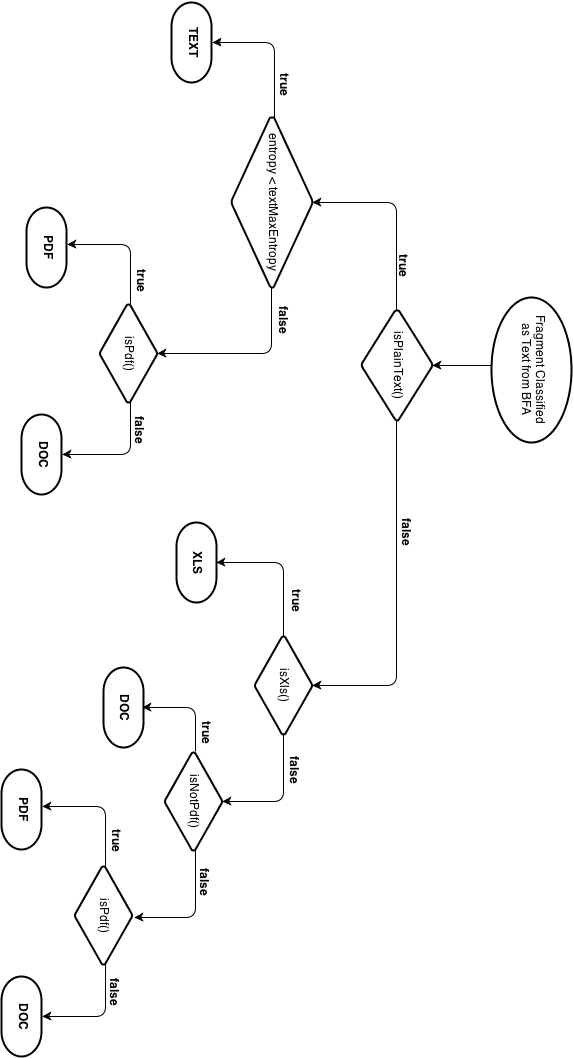
\includegraphics[scale=0.65]{./Figures/flowchart}
   \caption{Algorithm as Decision Tree\label{flowchart}}
\end{figure}


\chapter{Results}\label{chap:6}
In this chapter we are going to present the accuracy results of our classification algorithm. Analysis of the results will be presented in the next chapter.
Since our algorithms design is based on the analysis we did on the experimental data set(Table ~\ref{table:data set}), the algorithm is biased towards this set. For that reason we used the final testing data set(Table X) for testing our algorithms performance.

Although our final algorithm was implemented in one piece, we divide the results in three parts. In section ~\ref{sec:6.1} we  provide the performance of the first half of our algorithm, which is the BFA, regarding text fragment classification. In section ~\ref{sec:6.2} we provide the classification results of the algorithm we described in chapter~\ref{chap:5}. We should note that the classification results of that part correspond to the data set of fragments that were initially classified as text from the BFA.Finally, in section ~\ref{sec:6.3} we provide the final classification results of our complete algorithm. 
\pagebreak

\section{BFA Scan - Text Fragment Classification}\label{sec:6.1}
In Table \ref{table:final_bfa} we present the performance of the first part of our algorithm regarding text fragment classification. The first row corresponds to the initial number of fragments our algorithm processed for each file type. The second and the third row provide information regarding the amount of fragments that were classified as text from BFA.
%%------------------------------------------------------------------------------------------------------------------------------
\begin{table}[H]
\centering
\caption{BFA Text Fragments Classification\label{table:final_bfa}}
\colorbox{blue!25}{
\scalebox{0.65}{

\begin{tabular}{ l c c c c c c c c c c }
\hline
\hline
 & pdf & text & doc & xls & ppt  & mp4 & ogg & zip & png & jpg  \\ 
\hline
num. of fragments  & 1,874,910 & 1,891,472 & 1,775,747 & 1,870,376 & 1,864,145 & 1,888,605  & 1,891,754 & 1,889,477 & 1,880,742 & 1,886,853 \\[0.6ex]
\hline
\\[0.2ex]
fragments classified as text & 385,616 & 1,889,662  & 950,308 & 1,756,200 & 404,198 & 67,107 & 111,738 & 94,815 & 86,017 & 98,960     \\[0.6ex]
 \multicolumn{1}{r}{\%}   & 20.6  & 99.9  & 53.5 & 93.9 & 21.7 & 3.6 & 5.9 & 5 & 4.6 & 5.2     \\[0.6ex]
 
 fragments classified as other & 1,489,294  &1,810  & 825,439 & 114,176 & 1,459,947 & 1,821,498  & 1,780,016  & 1,794,662  & 1,794,725  & 1,787,893 \\[0.6ex]
 \multicolumn{1}{r}{\%}   & 79.4 & 0.1  & 46.5  &  6.1 & 78.3 & 96.4  & 94.1  & 95 & 95.4  & 94.8     \\\\[0.6ex]



\end{tabular}}}
\end{table}
%End sample table




\section{BFA Extension Algorithm Accuracy}\label{sec:6.2}
In Table \ref{table:final} we provide the accuracy results of our custom  algorithm as a percentage confusion matrix. The columns represent the actual type of the fragments while the rows represent the file type that the fragments was classified as. Since our algorithm was designed to classify fragments of the doc, pdf, xls and text file formats, we only have true positives percentages for these 4 file types. We present the true positive rates as shaded cells.

%%------------------------------------------------------------------------------------------------------------------------------
\begin{table}[H]
\centering
\caption{BFA Extension Algorithm Accuracy\label{table:final}}
\colorbox{blue!25}{
\scalebox{0.65}{

\begin{tabular}{ l c c c c c c c c c c }
\hline
\hline
 & pdf & text & doc & xls & ppt  & mp4 & ogg & zip & png & jpg  \\ 
\hline
fragments classified as text from BFA & 385,616 & 1,889,662  & 950,308 & 1,756,200 & 404,198 & 67,107 & 111,738 & 94,815 & 86,017 & 98,960     \\[0.6ex]
\hline
\\[0.2ex]
pdf 		 &\cellcolor{blue!15} 46.3  & 0.5  & 16.2  & 2.3   & 31.2  & 87.6  & 95.5 & 90.6  & 84.9& 83.0    \\[0.6ex]
text		 & 38.9  &\cellcolor{blue!15} 98.8    & 11.7  & 3.9   & 1.2   & 0     & 0.1   & 0  & 2.2 & 6.4\\[0.6ex]
doc 		 & 13.6  & 0.7   &\cellcolor{blue!15} 60.7  & 17.9  & 43.4  & 12.4  & 4.4  & 9.3 & 8.8 & 8.7   \\[0.6ex]
xls 		 & 1.3   & 0     & 11.4  &\cellcolor{blue!15} 75.9  & 24.2  & 0.1   & 0    & 0.2    & 4.1 & 2 \\[0.6ex]


\end{tabular}}}
\end{table}
%End sample table
\newpage
\section{Complete Algorithm Accuracy}\label{sec:6.3}
In Table \ref{table:final} we provide the accuracy results of our complete algorithm as a percentage confusion matrix. The columns represent the actual type of the fragments while the rows represent the file type that the fragments was classified as. Our algorithms can take 5 classification decisions. These decisions can be doc, pdf, xls, text and other. The "other" classification means that a fragment was classified as ppt, ogg, mp4, zip, png or jpg.  We present the true positive rates as shaded cells.
%%------------------------------------------------------------------------------------------------------------------------------
\begin{table}[H]
\centering
\caption{Algorithm Accuracy Results\label{table:overral_final}}
\colorbox{blue!25}{
\scalebox{0.7}{

\begin{tabular}{ l c c c c c c c c c c }
\hline
\hline
 & pdf & text & doc & xls & ppt  & mp4 & ogg & zip & png & jpg  \\ 
\hline
num. of fragments & 1,874,910  & 1,891,472  & 1,775,747  & 1,870,376  & 1,864,145  & 1,888,605 & 1,891,754  &1,889,477  & 1,880,742 
 & 1,886,853    \\[0.6ex]
\hline
\\[0.2ex]
pdf 		 &\cellcolor{blue!15}9.5   & 0.5 & 8.7 & 2.2 & 6.8  & 3.1   & 5.6  & 4.5   & 3.9 & 4.4   \\[0.6ex]
text		 & 8.0  &\cellcolor{blue!15} 98.8    & 6.3  & 3.7  & 0.2  & 0     & 0   & 0  & 0.1 & 0.3\\[0.6ex]
doc 		 & 2.8 & 0.7  &\cellcolor{blue!15} 32.5  & 16.8 & 9.4  & 0.4  & 0.3  & 0.5 & 0.4 & 0.5  \\[0.6ex]
xls 		 & 0.3   & 0     & 6.1  &\cellcolor{blue!15} 71.3  & 5.3 & 0  & 0    & 0   & 0.2 & 0.1 \\[0.6ex]
other	 & 79.4   & 0.1    & 46.5  & 6.1  &\cellcolor{blue!15}78.3   & \cellcolor{blue!15}96.4  &\cellcolor{blue!15}94.1 &\cellcolor{blue!15}95.0   & \cellcolor{blue!15}95.4 & \cellcolor{blue!15}94.8 \\[0.6ex]

\end{tabular}}}
\end{table}

\chapter{Results}\label{chap:6}
In this chapter we are going to present the accuracy results of our classification algorithm. Analysis of the results will be presented in the next chapter.
Since our algorithms design is based on the analysis we did on the experimental data set(Table ~\ref{table:data set}), the algorithm is biased towards this set. For that reason we used the final testing data set(Table X) for testing our algorithms performance.

Although our final algorithm was implemented in one piece, we divide the results in two parts. In section ~\ref{sec:6.1} we  provide the performance of the first half of our algorithm, which is the BFA, regarding text fragment classification. In section ~\ref{sec:6.2} we provide the final classification results of our complete algorithm. We should note that the final classification results correspond to the data set that is comrpised of fragments that were initially classified as text from the BFA.
\pagebreak

\section{BFA Scan - Text Fragment Classification}\label{sec:6.1}
In Table \ref{table:final_bfa} we present the performance of the first part of our algorithm regarding text fragment classification. The first row corresponds to the initial number of fragments our algorithm processed for each file type. The second and the third row provide information regarding the amount of fragments that were classified as text from BFA.
%%------------------------------------------------------------------------------------------------------------------------------
\begin{table}[H]
\centering
\caption{BFA Text Fragments Classification\label{table:final_bfa}}
\colorbox{blue!25}{
\scalebox{0.65}{

\begin{tabular}{ l c c c c c c c c c c }
\hline
\hline
 & pdf & text & doc & xls & ppt  & mp4 & ogg & zip & png & jpg  \\ 
\hline
num. of fragments  & 1,874,910 & 1,891,472 & 1,775,747 & 1,870,376 & 1,864,145 & 1,888,605  & 1,891,754 & 1,889,477 & 1,880,742 & 1,886,853 \\[0.6ex]
\hline
\\[0.2ex]
fragments classified as text & 385,616 & 1,889,662  & 950,308 & 1,756,200 & 404,198 & 67,107 & 111,738 & 94,815 & 86,017 & 98,960     \\[0.6ex]
 \multicolumn{1}{r}{\%}   & 20.6  & 99.9  & 53.5 & 93.9 & 21.7 & 3.6 & 5.9 & 5 & 4.6 & 5.2     \\[0.6ex]
 
 fragments classified as other & 1,489,294  &1,810  & 825,439 & 114,176 & 1,459,947 & 1,821,498  & 1,780,016  & 1,794,662  & 1,794,725  & 1,787,893 \\[0.6ex]
 \multicolumn{1}{r}{\%}   & 79.4 & 0.1  & 46.5  &  6.1 & 78.3 & 96.4  & 94.1  & 95 & 95.4  & 94.8     \\\\[0.6ex]



\end{tabular}}}
\end{table}
%End sample table




\section{Algorithm Accuracy}\label{sec:6.2}
In Table \ref{table:final} we provide the final accuracy results of our algorithm as a percentage confusion matrix. The columns represent the actual type of the fragments while the rows represent the file type that the fragments was classified as. Since our algorithm was designed to classify fragments of the doc, pdf, xls and text file formats, we only have true positives percentages for these 4 file types. We present the true positive values as shaded cells.

%%------------------------------------------------------------------------------------------------------------------------------
\begin{table}[H]
\centering
\caption{BFA Extension Algorithm Accuracy\label{table:final}}
\colorbox{blue!25}{
\scalebox{0.65}{

\begin{tabular}{ l c c c c c c c c c c }
\hline
\hline
 & pdf & text & doc & xls & ppt  & mp4 & ogg & zip & png & jpg  \\ 
\hline
fragments classified as text from BFA & 385,616 & 1,889,662  & 950,308 & 1,756,200 & 404,198 & 67,107 & 111,738 & 94,815 & 86,017 & 98,960     \\[0.6ex]
\hline
\\[0.2ex]
pdf 		 &\cellcolor{blue!15} 46.3  & 0.5  & 16.2  & 2.3   & 31.2  & 87.6  & 95.5 & 90.6  & 84.9& 83.0    \\[0.6ex]
text		 & 38.9  &\cellcolor{blue!15} 98.8    & 11.7  & 3.9   & 1.2   & 0     & 0.1   & 0  & 2.2 & 6.4\\[0.6ex]
doc 		 & 13.6  & 0.7   &\cellcolor{blue!15} 60.7  & 17.9  & 43.4  & 12.4  & 4.4  & 9.3 & 8.8 & 8.7   \\[0.6ex]
xls 		 & 1.3   & 0     & 11.4  &\cellcolor{blue!15} 75.9  & 24.2  & 0.1   & 0    & 0.2    & 4.1 & 2 \\[0.6ex]


\end{tabular}}}
\end{table}
%End sample table
\chapter{Analysis}
In this chapter we will analyse the results of chapter \ref{chap:6}. We divide this chapter in three sections. In section \ref{sec:7.1} we analyse the performance of BFA and the amount of fragments that were classified as text. In section  \ref{sec:7.2} we analyse the performance of our complete algorithm. Finally in section  \ref{sec:7.3} we compare our algorithm performance with the classification algorithms that Shahi tested in \cite{Shahi}.

\section{BFA performance}\label{sec:7.1}
In our final test, the BFA part of our algorithm performed as expected. It yielded almost identical results as the results that we got during the algorithms development procedure (chapter \ref{chap:6}).

In a corpus of 18.714.081 fragments BFA classified 5.844.621 as text. From that amount 4.981.786 of fragments do originate from document-type fragments and 862.835 from the other 6 file types. This means that we have a percentage of 85,2\% true positives and a 14,8\% of false positives regarding text fragment classification. These results are in pair with the ones that we got when we used this variation of BFA in a ten-times smaller corpus(Table \ref{table:table 4.1}).

Moreover, this 85,2\% of true positives correspond to the 67,2\% of the total doc, pdf, xls and text fragments of our initial corpus. However, this percentage is not representative for a real life case, since our final testing set was comprised only of fragments that had at least one plain text character. Considering that we know for each one of the 10 file types that we use the percentage of fragments that contain np plain text(Tables ~\ref{data set}~\ref{table:final set}, we can calculate the approximate overall document-type fragment retrieval in a corpus of 10GB size. Thus, taking under account the amount of fragments that correspond to fragments with 0\% plain text concentration, the BFA would have approximately retrieved the 63\% of the total doc, pdf, xls and text fragments from a 10GB corpus.

\section{Overall Algorithm Performance}\label{sec:7.2}
The accuracies for the 4 file types of our interest are quite encouraging. We got 9,5\% for pdf, 98,8\% for text, 32,5\% for doc, 71,3\% for xls fragments and 92,4\% for classifying a fragments as of another file type. It seems that due to the high entropy of the non-document type fragments, most of the fragments that were initially falsely classified as text, thereafter were falsely classified as pdf. This is not necessarily a bad thing, since it kept in low levels the false positives rates for the doc, xls and text file types. Especially for the text and xls file types the false positive rates are extremely small.

However, the information that we can get from this results are insufficient to evaluate our algorithms performance. In addition, this is the main problem with the scientific publications in the file carving field. We observed that most of the papers upon file carving techniques provide only the true positive rates and doesn't give more information regarding the classification capacity of their algorithms. Surprisingly enough, this is in general a common phenomenon in algorithm comparison studies \cite{Demsar}\cite{Sokolova}.

We consider that by calculating the $F-score$ along with the overall accuracy of our algorithm we can acquire better insight for our algorithms performance. The $F-score$  is a statistical measure that tests accuracy and it considers both the precision and recall  measures of the test to compute the score. A higher $F-score$ implies higher accuracy. The $F-score$ measurement is described in formula ~\ref{formula:fscore}. Note that $tp$ stands for "true positive", $fp$ for "false positive", $tn$ for "true negative" and $fn$ for "false negative".




\noindent\begin{minipage}{.5\linewidth}
\small

\begin{equation}
precision = \frac{tp}{tp + fp}
\end{equation}
\end{minipage}%
\begin{minipage}{.5\linewidth}
\small
\begin{equation}
recall = \frac{tp}{tp + fn}
\end{equation}
\end{minipage}%

\begin{center}
\begin{minipage}{.5\linewidth}
\small
\begin{equation}
\newline
F-score = 2 * \frac{precision * recall}{precision + recall}
\end{equation}
\label{formula:fscore}
\end{minipage}
\end{center}

Additionally, the equation that we use to calculate overall accuracy can be found in formula \ref{overall_accuracy}. *** FIx link numbers***

\begin{center}
\noindent\begin{minipage}{.5\linewidth}
\small
\begin{equation}
overall \ accuracy = \frac{correct\ predictions}{total\ predictions}  
\end{equation}
\label{overall_accuracy}
\end{minipage}
\end{center}

The results of the aforementioned measurements can be found in Table ~\ref{table:overall_results}. Our classifier performed extremely well for the text and xls file types with an ${F_1}-score$ of 0,91 and 0,78 respectively. The prediction rates  for the doc file type are quite satisfying with an ${F_1}-score$  of 0,39. We say quite satisfying considering that the doc file type was the most "tricky" among the document-file types we analysed, due to the fact that we couldn't find strong distinctive characteristics. Furthermore, the worst rates are for the pdf file type, mainly because BFA classified as text only the 20\% of the initial pdf fragments. Additionally, during the second phase of our classification algorithm most of non-document type fragments were falsely classified as pdf due to their high entropy. Finally, the overall accuracy of our classifier is 0,77, a very high number for a file carving technique. This means that in 100 predictions, 77 of them will be correct.
\begin{table}[H]
\centering
\caption{Algorithm Prediction Rates}
\label{table:overall_results}
\colorbox{blue!25}{

\begin{tabular}{ l c c c c c c c c c c }
\hline
\hline

                 & pdf   &  text  &  doc  &  xls  & other\\ 
\hline
\\[0.2ex]
precision 		 & 0,1  &  0,85  & 0,49   & 0,86  & 0,81  \\[0.8ex]
$F-score$	 & 0,1  &  0,91  & 0,39   & 0,78  & 0,86    \\\\[0.8ex]

overall accuracy:  & 0,77 &  &  &     \\ [0.8ex]

\end{tabular}}
\end{table}

\section{Algorithm Comparison}
In this section we try to compare the performance of our classifier with similar classification techniques. In subsection ~\ref{sub:accuracy} we compare the accuracies of the algorithms and in subsection ~\ref{sub:speed} we compare their performance in terms of execution time.

Among the algorithms that we compare are the Byte Frequency Analysis algorithm\cite{MacDaniel}, the n-Gram Analysis\cite{ngram}, the Rate of Change\cite{roc} and the algorithm of Conti et al.\cite{Conti}. We use the results that Shahi acquired from his experiment\cite{Ashim}. We chose to compare our algorithms performance with Shahis results, because he used the same file types for his experiment. Additionally, his testing set was of the exact same size as the one we used for our final testing set. One of the major problems in the file carving field is that there is no proper comparison between classification algorithms, since every technique was tested in different data sets that were comprised of different file types. Furthermore, at this point we should note that for the comparison of the algorithms , we use the results that Shahi got by using fingerprints that were trained with the 10\% of his total training set. This 10\% corresponds to the size of the training set that we used to train our fingerprints.


\subsection{Accuracy Comparison}\label{sub:accuracy}
Although the testing sets that were used for all the experiments are similar, it is still quite difficult to compare these algorithms. Our algorithm was specifically designed to classify only fragments of 4 file types or to classify as "other" everything that was classified as non-text from its BFA part. Moreover, all algorithms do not give an $F-score$ for every file type. The results can be found in Table ~\ref{comparison_table}.

\begin{table}[H]
\centering
\caption{Classification Algorithm Accuracy Comparison}
\label{comparison_table}
\colorbox{blue!25}{
\scalebox{0.8}{
\begin{tabular}{ l c c c c c c c c c c c c r }
\hline
\hline

 & pdf  &  zip  &  text  &  doc  &  mp4  &  xls  &  ppt  &  jpg  &  ogg  &  png & other &&overall accuracy  \\ 
\hline
\\[0.2ex]
Our algorithm 		     & 0,1  & -   & 0,91  & 0,39   & -     & 0,78   &  -  & -  & -  & - & 0,86 &\ & 0,77 \\[0.8ex]

Byte Frequency Analysis 	 & - & 0,42   & 0,59  & 0,01  & 0,25    & 0,54   &  -    & 0,16    &0,17  & 0,17 & -&\ & 0,33 \\[0.8ex]

Rate of Change		     & 0,37  & -   & 0,73  & 0,5  & -     & 0,8   &  0,22    & -     & -  & - &- &\ & 0,32 \\[0.8ex]

n-Gram Analysis		     & 0,17 & -  & 0,89  & 0,12  & -    & 0,74  &  0,22   & -    &- & - & -&\ & 0,30 \\[0.8ex]

Algorithm of Conti et al.  & 0,10 & 0,46  & 0,44  & 0,16  & 0,37    & 0,38  &  0,06    & 0,23    & 0,16 & 0,08 & -&\ & 0,30 \\[0.8ex]




\end{tabular}}}
\end{table} 

Our algorithm outperforms the other 4 in classifying fragments of the text file format with an $F-score$ of 0,91. Furthermore, it comes second only after the Rate of Change algorithm regarding xls and doc fragment classification. Lastly, the $F-score$ for the pdf file types is the worst along with the algorithm of Conti et al. score. Moreover, our algorithms overall accuracy is approximately 2,5 times higher than the overall accuracies of the other algorithms. However, we should not forget that our algorithm is limited in classifying only fragments that contain at least one plain text character. Overall, although our algorithm takes less decisions and classifies non-document fragments in a broad class, its decisions are significantly more reliable than the decisions of its competitors.

\subsection{Execution Time Comparison}\label{sub:speed}




\chapter{Discussion}
In our experiment, during our algorithm development procedure our analysis yielded two new classification metrics. The Individual Null Byte Frequency(INBF) and the Plain Text Concentration(PTC). The representative INBF values that we used to classify mainly document-type fragments were formed from BFAs output. The output was comprised only of fragments that were classified as text from BFA. This resulted to an unpropitious set of fragments of the 4 document-type file formats. The amount of pdf and doc fragments were significantly less than the amount of text and xls. Although INBF seems to be quite effective as a part of our classification algorithm, we believe that a more extensive analysis must be made in a bigger data set, in order to be able to say if this metric could provide aid for broad fragment classification. On the other hand, PTC analysis was made in a corpus of 10GB in total and we believe that our analysis is consistent and can be a great asset in file carving techniques.

Although we did our best to eliminate possible biases in our experimental setup, we can not guarantee the integrity of our corpus. Considering that our corpus was comprised of tens of thousands of files it wasn't feasible to manually check if the suffixes of the files correspond to the actual file type. We did some manual inspections in the experimental data set and we found about 30mbs of files that had a $.txt$ suffix but weren't text files. Additionally, we don't know if our corpus was comprised of various file format versions. For example, an Adobe PDF 1.7 document might be slightly different from an Adobe PDF 1.3 document.
\chapter{Appendix}

\section{test}
\begin{table}[t]
\centering
\caption{BFA - Fingerprints Trained in 0-25\% and tested in 0-25\%\label{table:table 4.3}}
\colorbox{blue!30}{
\scalebox{0.75}{

\begin{tabular}{ l c c c c c c c c c c }
\hline
\hline
 & pdf  &  zip  &  text  &  doc  &  mp4  &  xls  &  ppt  &  jpg  &  ogg  &  png \\ 
\hline
num.of fragments  & \ 5,714 \  &\ \ \ 90 \ \  & \ \ \ \ \ 3 \ \ \  & \ 52,264   &\ 2,854 \  & 147,873   & \ 11,027   & \ 1,332 \   &\ \  222 \ \  & \ 7,874 \   \\[0.6ex]
\hline
\\[0.2ex]
pdf 		 &\cellcolor{blue!15}0   & 0   & 0  & 0  & 0  & 0.3 & 0  & 0.1   & 0    & 0   \\[0.6ex]
zip 		 & 0  & \cellcolor{blue!15}0   & 0  & 0  & 0  & 0   & 0  & 0   & 0.5        & 0   \\[0.6ex]
\rowcolor{blue!50}
\cellcolor{blue!30}text & 0  & 0  & \cellcolor{blue!15}0 & 0.1   & 0  & 0.7   & 0  & 0  & 0   & 0 \\[0.6ex]
doc 		 & 0     & 0    & 0     & \cellcolor{blue!15}0  & 0   & 0   & 0   & 0.1    & 0   & 0   \\[0.6ex]
mp4 		 & 0     & 0    & 0     & 0  &\cellcolor{blue!15}0.1  & 0.1   & 0   & 0 & 0  & 0    \\[0.6ex]
xls 		 & 99.6  & 95.6 & 100   & 99.6   & 99.9   & \cellcolor{blue!15}97.3  & 98.3   & 95.3  & 96.3   & 99.9   \\[0.6ex]
ppt 		 & 0     & 0    & 0     & 0      & 0      & 0 & \cellcolor{blue!15}0  & 0  & 0 & 0   \\[0.6ex]
jpg 		 & 0.3   & 4.4  & 0     & 0.2    & 0      & 0.9  & 1.6   & \cellcolor{blue!15}4.5   & 2.7   & 0.1  \\[0.6ex]
ogg 		 & 0     & 0    & 0     & 0      & 0      & 0.2  & 0  & 0.1   & \cellcolor{blue!15}0  & 0   \\[0.6ex]
png 		 & 0     & 0    & 0     & 0      & 0      & 0.4  & 0  &   & 0.5   &\cellcolor{blue!15}0  \\[0.6ex]
Unclassified  &  0  & 0  & 0  & 0  & 0  & 0  & 0  & 0  & 0  & 0   \\[0.6ex]
\end{tabular}}}
\end{table}



\begin{table}[b]
\centering
\caption{BFA - Fingerprints Trained in 25-50\% and tested in 25-50\%\label{table:table 4.4}}
\colorbox{blue!30}{
\scalebox{0.75}{
\begin{tabular}{ l c c c c c c c c c c }
\hline
\hline
 & pdf  &  zip  &  text  &  doc  &  mp4  &  xls  &  ppt  &  jpg  &  ogg  &  png \\ 
\hline
num.of fragments  & 147,705 	 & 204,662  &\ \ 285 \ \   & 102,831   &  201,859  & \ 41,013   & 178,816  & 193,103   & 195,368   & 187,688    \\[0.6ex]
\hline
\\[0.2ex]
pdf 		 & \cellcolor{blue!15}6.9  & 4  & 4.9   & 5.5   & 5.1  & 0.1  & 6    & 5.8   & 5.2   & 5.3    \\[0.6ex]
zip 		 & 25.2 &\cellcolor{blue!15}26.7  & 14  & 23.7  & 28.4 & 0.6  & 27.6 & 30    & 25.3  & 29.5   \\[0.6ex]
\rowcolor{blue!50}
\cellcolor{blue!30}text	& 32.6  & 40.1 &\cellcolor{blue!15}14.7 & 30.9   & 38.8   & 0.8  & 33.4  & 34.7  & 36.5   & 37.3  \\[0.6ex]
doc 		 & 16.3  & 17.7  & 4.9   & \cellcolor{blue!15}15.6  & 15.8  & 0.4   & 14.8   & 14.4   & 19.4   & 15.1    \\[0.6ex]
mp4 		 & 2     & 0.8   & 2.1   & 1.1   & \cellcolor{blue!15}1.7   & 0   & 1.2   & 1.1  & 1.1   & 1.1   \\[0.6ex]
xls 		 & 3.9   & 1.7   & 49.1  & 11.5  & 0    & \cellcolor{blue!15}97.9  & 4.2  & 0.8  & 1.3   & 0.4   \\[0.6ex]
ppt 		 & 9.2   & 6.7   & 7.7   & 8.8   & 7.4  & 0.2  & \cellcolor{blue!15}9.5   & 9.8  & 8.1   & 8.6   \\[0.6ex]
jpg 		 & 0.7   & 0.3   & 0.7   & 0.5   & 0.2  & 0    & 0.6   & \cellcolor{blue!15}0.6  & 0.4   & 0.4  \\[0.6ex]
ogg 		 & 2.6   & 1.5   & 1.8   & 2     & 2.2  & 0.1  & 2.2   & 2.2   & \cellcolor{blue!15}2.2  & 2   \\[0.6ex]
png 		 & 0.6   & 0.3   & 0     & 0.5   & 0.4  & 0    & 0.6   & 0.5   & 0.5   & \cellcolor{blue!15}0.5  \\[0.6ex]
Unclassified  &  0  & 0  & 0  & 0  & 0  & 0  & 0  & 0  & 0  & 0   \\[0.6ex]
\end{tabular}}}
\end{table}

%%------------------------------------------------------------------------------------------------------------------------------
\begin{table}[!]
\centering
\caption{BFA - Fingerprints Trained in 50-75\% and tested in 50-75\%\label{table:table 4.5}}
\colorbox{blue!30}{
\scalebox{0.75}{

\begin{tabular}{ l c c c c c c c c c c }
\hline
\hline
 & pdf  &  zip  &  text  &  doc  &  mp4  &  xls  &  ppt  &  jpg  &  ogg  &  png \\ 
\hline
num.of fragments  & 12,421	 & 43 & 1,203   & 2,101   & 15   & 3,158   & 2,393   & 147  & 66   & 89    \\[0.6ex]
\hline
\\[0.2ex]
pdf 		 & \cellcolor{blue!15}39.1  & 23.3   & 6.2  & 1.8   & 0  & 1.6  & 1.6  & 2   & 3   & 1.1    \\[0.6ex]
zip 		 & 4.8  & \cellcolor{blue!15}16.3    & 6.7  & 10.4  & 0  & 0.4  & 3.1  & 5.4  & 1.5  & 14.6   \\[0.6ex]
\rowcolor{blue!50}
\cellcolor{blue!30}text		 & 0.6  & 2.3  & \cellcolor{blue!15}1.6  & 5.9   & 0  & 0   & 2.3  & 2  & 0   & 9  \\[0.6ex]
doc 		 & 6.2  & 7   & 40.9   & \cellcolor{blue!15}7.5  & 0  & 2.4  & 18.2  & 4.1   & 3  & 1.1    \\[0.6ex]
mp4 		 & 12.2 & 27.9  & 1.2  & 37.6 & \cellcolor{blue!15}100  & 27.2   & 42.6   & 40.8  & 36.4  & 12.4   \\[0.6ex]
xls 		 & 13.5 & 0   & 1.4    & 19.6   & 0   & \cellcolor{blue!15}65.5  & 18.7   & 35.4   & 15.2   & 1.1   \\[0.6ex]
ppt 		 & 16.0 & 0   & 17.5   & 1.4    & 0   & 1.5  & \cellcolor{blue!15}0.6  & 0.7  & 1.5  & 0  \\[0.6ex]
jpg 		 & 5.3  & 0   & 15.1   & 1.2    & 0   & 1.2  & 7  &\cellcolor{blue!15}1.4  & 3   &3.4   \\[0.6ex]
ogg 		 & 0.6  & 0   & 8.8    & 3.7    & 0   & 0.2  & 4.9   & 0   & \cellcolor{blue!15}36.4  & 0    \\[0.6ex]
png 		 & 1.5  & 23.3  & 0.5  & 10.9   & 0   & 0  & 0.9     & 8.2  & 0   & \cellcolor{blue!15}57.3  \\[0.6ex]
Unclassified  &  0  & 0  & 0  & 0  & 0  & 0  & 0  & 0  & 0  & 0   \\[0.6ex]
\end{tabular}}}
\end{table}
%End table - BFA Results only 50-75% Ratios

%%------------------------------------------------------------------------------------------------------------------------------
\begin{table}[!]
\centering
\caption{BFA - Fingerprints Trained in 75-100\% and tested in 75-100\%\label{table:table 4.6}}
\colorbox{blue!30}{
\scalebox{0.75}{

\begin{tabular}{ l c c c c c c c c c c }
\hline
\hline
 & pdf  &  zip  &  text  &  doc  &  mp4  &  xls  &  ppt  &  jpg  &  ogg  &  png \\ 
\hline
num.of fragments  & 23,892 &\ \ \ 0 \ \ \    & 188,564   & 20,691  & \ \ \ 0 \ \ \   & 1,308   & 3,053   & 1,026  & \ \ \ 0 \ \ \   & \ \ \ 2 \ \ \    \\[0.6ex]
\hline
\\[0.2ex]
pdf 		 & \cellcolor{blue!15}7.6  & 0  & 0.3  & 0.3  & 0  & 0   & 0.5  & 0   & 0   & 0    \\[0.6ex]
zip 		 & 0.7  & \cellcolor{blue!15}0  & 0.4  & 0.5  & 0  & 3.7 & 5.9  & 1.2 & 0   & 0   \\[0.6ex]
\rowcolor{blue!50}
\cellcolor{blue!30}text	 & 11.8  & 0  & \cellcolor{blue!15}1.4 & 3.4   & 0   & 6.2   & 2.3  & 1.8  & 0   & 0  \\[0.6ex]
doc 		 & 2     & 0  & 8.2   & \cellcolor{blue!15}43.2 & 0  & 17.7    & 5.3   & 1.4   & 0  & 0    \\[0.6ex]
mp4 		 & 49.3  & 0  & 86.5   & 48.6 & \cellcolor{blue!15}0  & 68.3   & 78.0  & 74.4  & 0  & 0   \\[0.6ex]
xls 		 & 7.9   & 0  & 0.6    & 1.2   & 0   & \cellcolor{blue!15}0.9  & 2.9   & 0.1   & 0  & 0  \\[0.6ex]
ppt 		 & 0.8   & 0  & 0.7    & 0.1   & 0   & 0   & \cellcolor{blue!15}0.3  & 0  & 0  & 100   \\[0.6ex]
jpg 		 & 4.2   & 0  & 1.4    & 1.7   & 0   & 1.3   & 0.8  & \cellcolor{blue!15}20.6  & 0  & 0   \\[0.6ex]
ogg 		 & 4.3   & 0  & 0.4    & 0.9   & 0   & 1.8   & 3.7  & 0.7   & \cellcolor{blue!15}0  & 0   \\[0.6ex]
png 		 & 11.4  & 0  & 0      & 0     & 0   & 0     & 0.4  & 0     & 0                     & \cellcolor{blue!15}0  \\[0.6ex]
Unclassified  &  0  & 0  & 0  & 0  & 0  & 0  & 0  & 0  & 0  & 0   \\[0.6ex]
\end{tabular}}}
\end{table}
%End table - BFA Results only 75-100% Ratios

%%This is the last chapter 
%%=========================================
\chapter[Summary]{Summary and Recommendations for Further Work}

In this final chapter you should sum up what you have done and which results you have got. You should also discuss your findings, and give recommendations for further work.

%%=========================================
\section{Summary and Conclusions}
Here, you present a brief summary of your work and list the main results you have got. You should give comments to each of the objectives in Chapter 1 and state whether or not you have met the objective. If you have not met the objective, you should explain why (e.g., data not available, too difficult).

This section is similar to the Summary and Conclusions in the beginning of your report, but more detailed---referring to the the various sections in the report.

%%=========================================
\section{Discussion}
Here, you may discuss your findings, their strengths and limitations.
%%=========================================
\section{Recommendations for Further Work}
You should give recommendations to possible extensions to your work. The recommendations should be as specific as possible, preferably with an objective and an indication of a possible approach.

The recommendations may be classified as:
\begin{itemize}
\item Short-term
\item Medium-term
\item Long-term
\end{itemize}
% Include more chapters as required.
%%=========================================
%\appendix

% Include more appendices as required.
%%=========================================
%\bibliographystyle{apa}
%\addcontentsline{toc}{chapter}{\bibname}
%\bibliography{refs}  
\begin{thebibliography}{99}
\bibitem{Aronson}      
Aronson, L., \& Bos, J. Van Den. (2011). Towards an Engineering Approach to File Carver Construction. 2011 IEEE 35th Annual Computer Software and Applications Conference Workshops, pp . 368–373.

\bibitem{MacDaniel}
M. McDaniel and M. Heydari , “ Content based file type detection algorithms ,” in Proc. 36th Annu. Hawaii Int. Conf. System Sciences (HICSS’03)—Track 9 , IEEE Computer Society , Washington , D.C. , 2003 , p. 332.1

\bibitem{Scalpel}
G. G. Richard , III and V. Roussev , “ Scalpel: A frugal, high performance file carver ,” in Proc. 2005 Digital Forensics Research Workshop (DFRWS) , New Orleans , LA , Aug. 2005 .

\bibitem{Pal}
Pal, A., \& Memon, N. (2009). The evolution of file carving. Signal Processing Magazine, IEEE, (March),pp. 59–71.

\bibitem{ngram}
W.J. Li , K. Wang , S. Stolfo , and B. Herzog , Fileprints: Identifying
file types by n-gram analysis , in Proc. 6th IEEE Systems, Man and
Cybernetics Information Assurance Workshop , 2005 , pp. 64 67.

\bibitem{Garfinkel}
Garfinkel, S. L. (2007). Carving contiguous and fragmented files with fast object validation. Digital Investigation, 4, pp. 2–12

\bibitem{Sceadan}
Maddox, L., \& Beebe, N. (2012). Systematic Classification Engine and Data Analysis Overview by Dr . Nicole Beebe

\bibitem{Ashim}
Shahi, A. Classifying the classifiers for file fragment classification, August 2012.

\bibitem{Shannon}
Shannon CE. The mathematical theory of communication. Bell System Tech J 1948;27:379–423, 623–56.

\bibitem{roc}
M. Karresand and N. Shahmehri, "File Type Identification of Data Fragments by their Binary Structure," in Proceedings of the 7th Annual IEEE Information Assurance Workshop, 2006.

\bibitem{Veenman}
C. Veenman, "Statistical Disk Cluster Classification for File Carving," in Proceedings of the First Internation Workshop on Computational Forensics, 2007.

\bibitem{Calhoun}
Calhoun, W. C., \& Coles, D. (2008). Predicting the types of file fragments. Digital Investigation, 5, S14–S20.


\bibitem{Axelsson}
Axelsson, S. (2010). The Normalised Compression Distance as a file fragment classifier. Digital Investigation, 7, S24–S31. doi:10.1016/j.diin.2010.05.004

\bibitem{Gopal}
Gopal S, Yang Y, Salomatin K, Carbonell J. Statistical learning for file-type identification. In: 2011 10th International Conference on Machine Learning and Applications and Workshops (ICMLA), Vol. 1; 2011. p. 68–73.

\bibitem{Fitz}
Fitzgerald, S., Mathews, G., Morris, C., \& Zhulyn, O. (2012). Using NLP techniques for file fragment classification. Digital Investigation, 9, S44–S49.

\bibitem{Conti}
Conti G, Bratus S, Sangster B, Ragsdale R, Supan M, Lichtenberg A, et al. Automated mapping of large binary objects using primitive fragment type classification. In: Proceedings of the 2010 Digital Forensics Research Conference (DFRWS); 2010.

\end{thebibliography}
%%=========================================
   
%%=============================================

\end{document}
